\providecommand{\rasd}{..}
\documentclass[../RASD.tex]{subfiles}

\begin{document}
    \chapter{User Interface Design}\label{ch:user-interface-design}
    In this chapter is given a general view about the structure of the application.
    A user flow diagram is presented to clarify the possible actions that a user can perform while using the application.
    This section is built according with the mockups presented in the RASD; regarding that, some windows has been added to better clarify
    the flow and to give a more complete idea of the user experience inside the application.
    \begin{figure}[H]
        \centering
        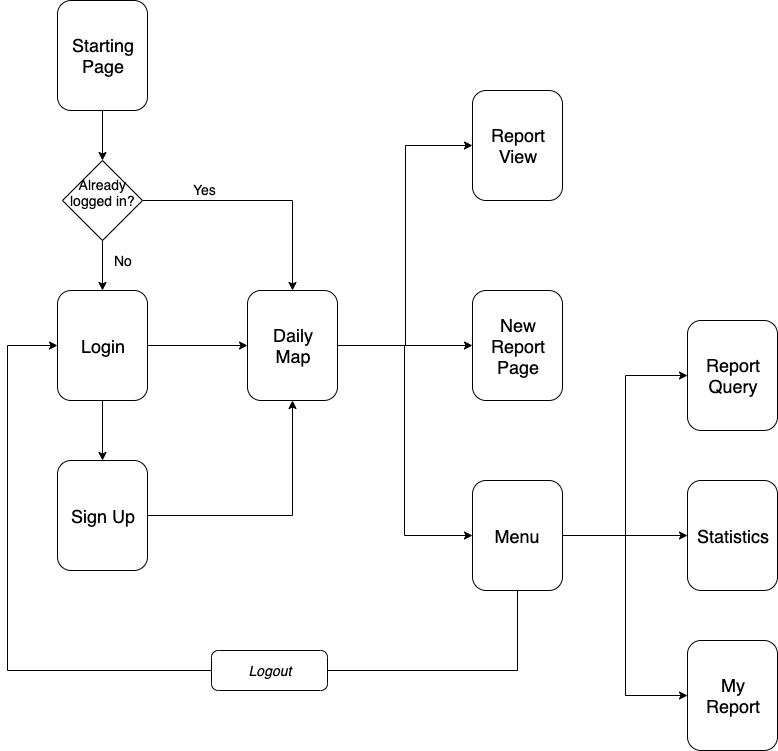
\includegraphics[scale = 1.5]{assets/ux.png}\\[1.6 cm]
        \caption[\textit{UX} Diagram]{UX diagram of the application.}
    \end{figure}
    It can be useful to analyze some aspects of the diagram.
    First of all, the starting page is not a real window of the application, but just denote the first page shown to the user after the application launch:
    in particular, if the user already used the application without logging out, he will directly see the daily map, otherwise if he logs out or if it is the first time
    that he uses the application on that device, the login page will be shown.
    Another important thing to notice is that the main page of the application is not the menu, but daily map, which is considered the core of the application itself.
    From this page will be than possible to switch to some related functionalities or to the main menu.
    It is important to clarify that this diagram wants to show the structure of SafeStreets, that will find a corresponding in the real application,
    but some more minor features not showed could be added later.
    \begin{figure}[H]
        \centering
        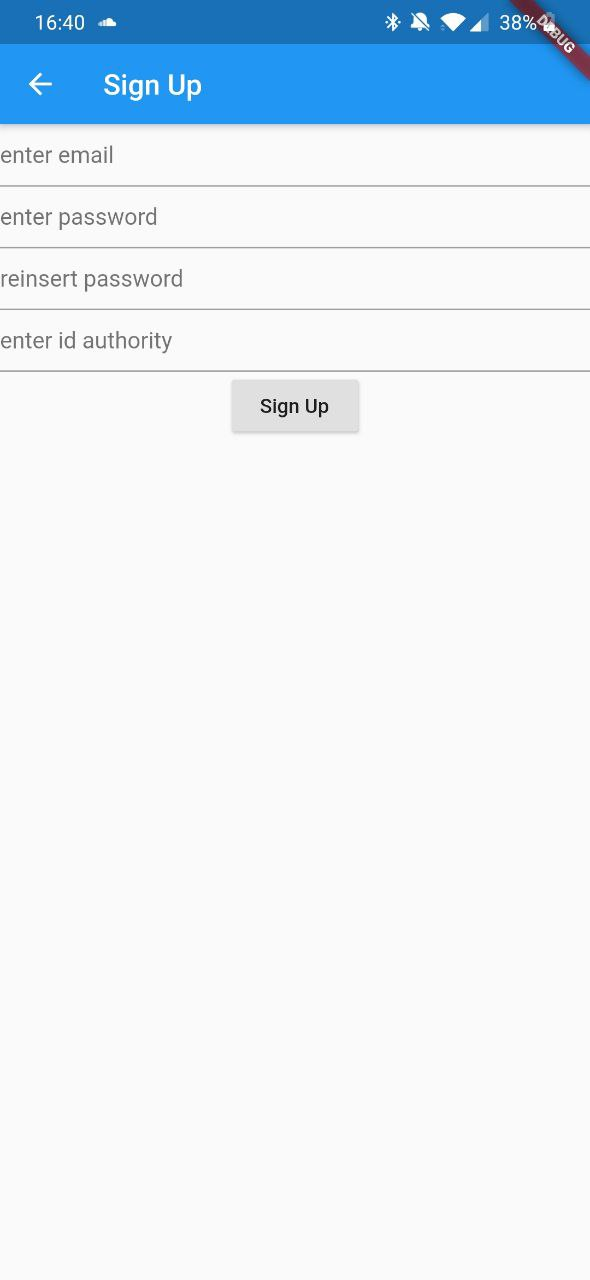
\includegraphics[scale = 0.2]{assets/app_screenshots/signup.jpg}\\[1.6 cm]
        \caption[\textit{Sign Up} Screenshot]{The registration page of SafeStreets.}
    \end{figure}
    \begin{figure}[H]
        \centering
        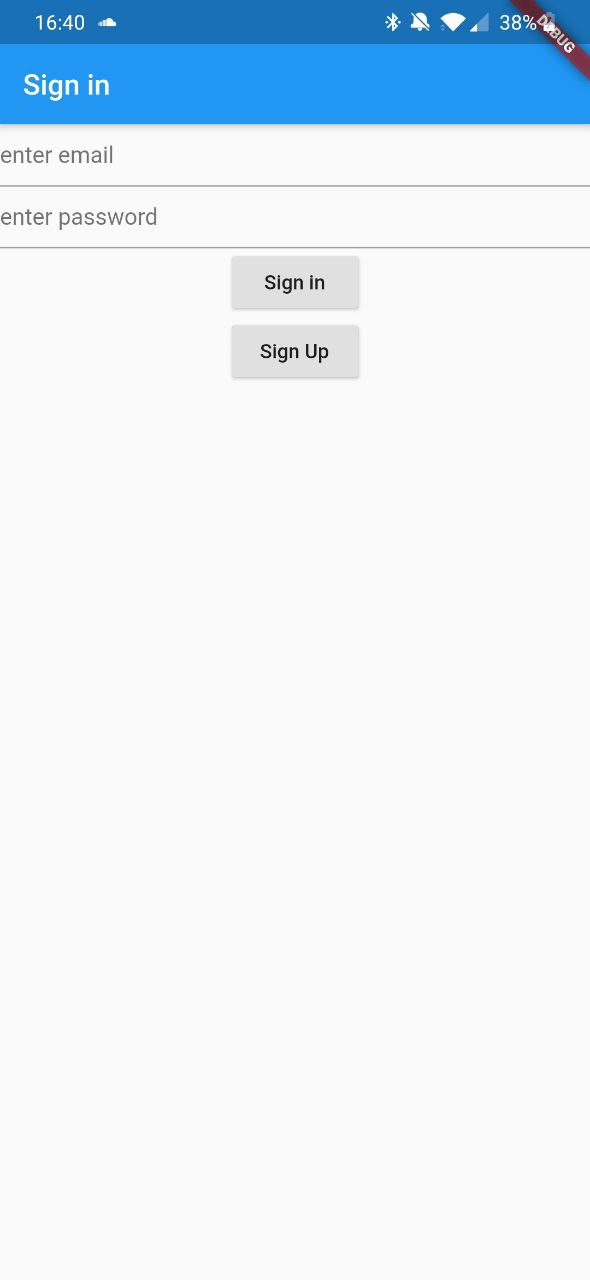
\includegraphics[scale = 0.2]{assets/app_screenshots/login.jpg}\\[1.6 cm]
        \caption[\textit{Login} Screenshot]{The login page of SafeStreets.}
    \end{figure}
    \begin{figure}[H]
        \centering
        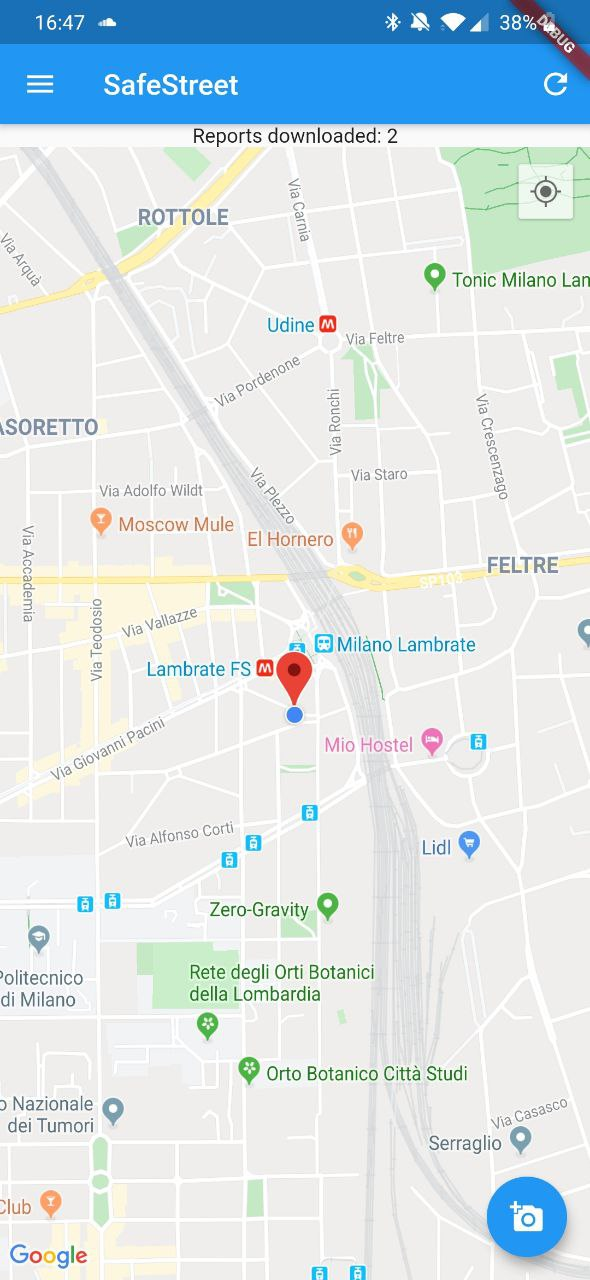
\includegraphics[scale = 0.2]{assets/app_screenshots/home.jpg}\\[1.6 cm]
        \caption[\textit{Home Page} Screenshot]{The homepage page of SafeStreets.}
    \end{figure}
    \begin{figure}[H]
        \centering
        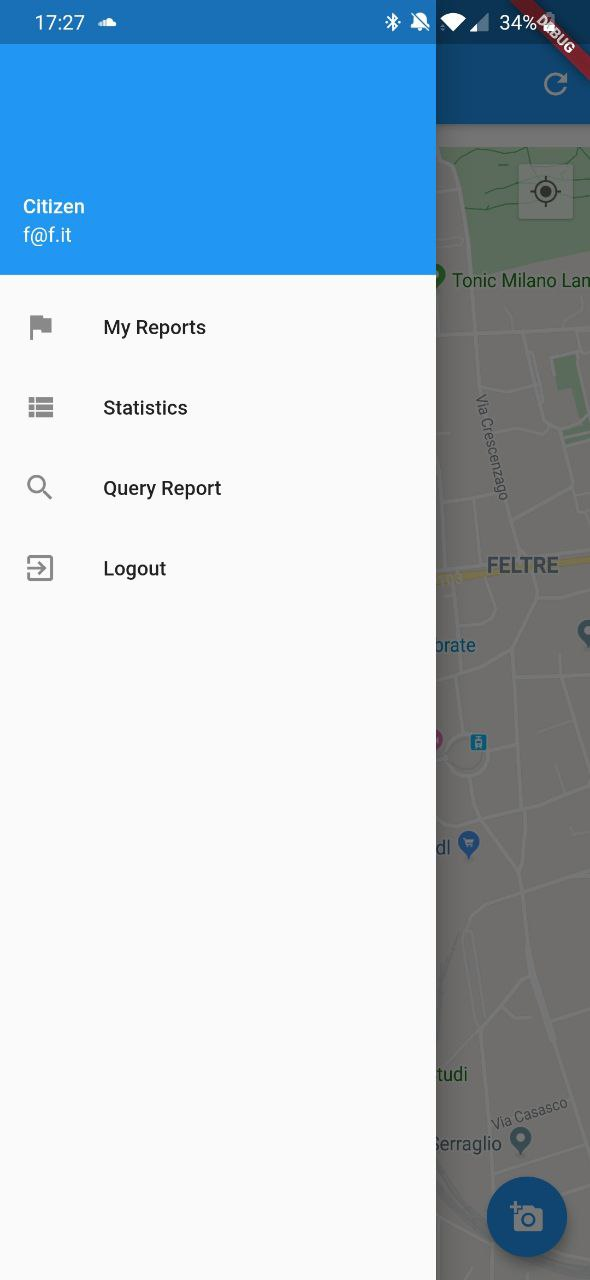
\includegraphics[scale = 0.2]{assets/app_screenshots/menu.jpg}\\[1.6 cm]
        \caption[\textit{Menu} Screenshot]{Menu drawer in SafeStreets.}
    \end{figure}
    \begin{figure}[H]
        \centering
        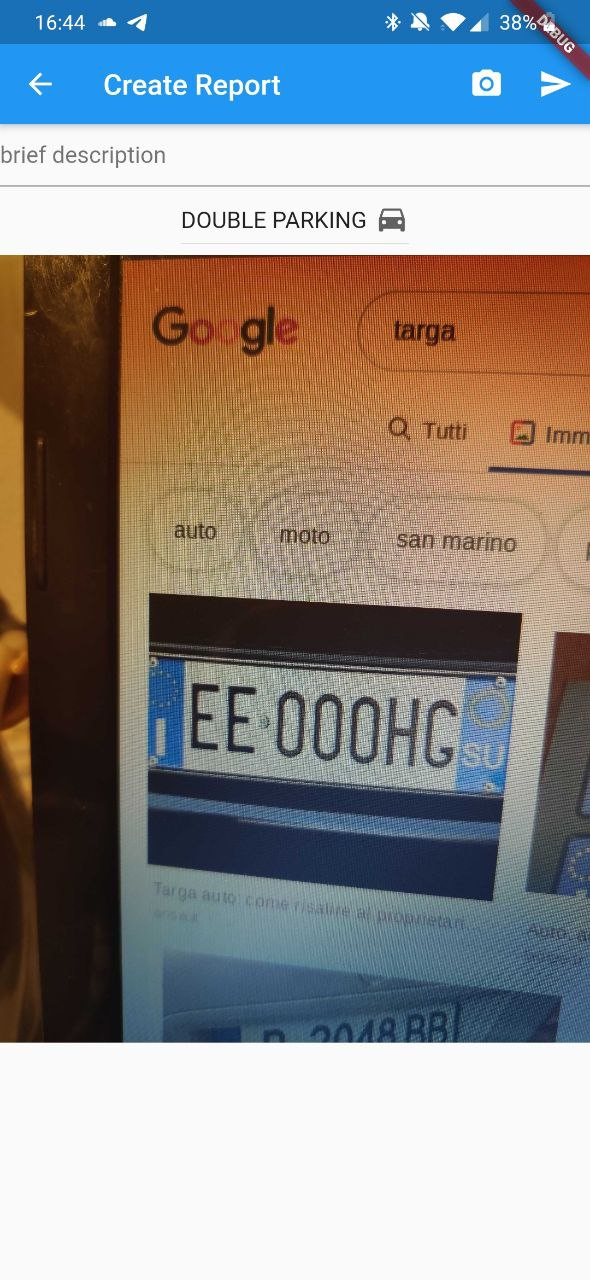
\includegraphics[scale = 0.2]{assets/app_screenshots/create.jpg}\\[1.6 cm]
        \caption[\textit{Create Report} Screenshot]{The create report page of SafeStreets.}
    \end{figure}
    \begin{figure}[H]
        \centering
        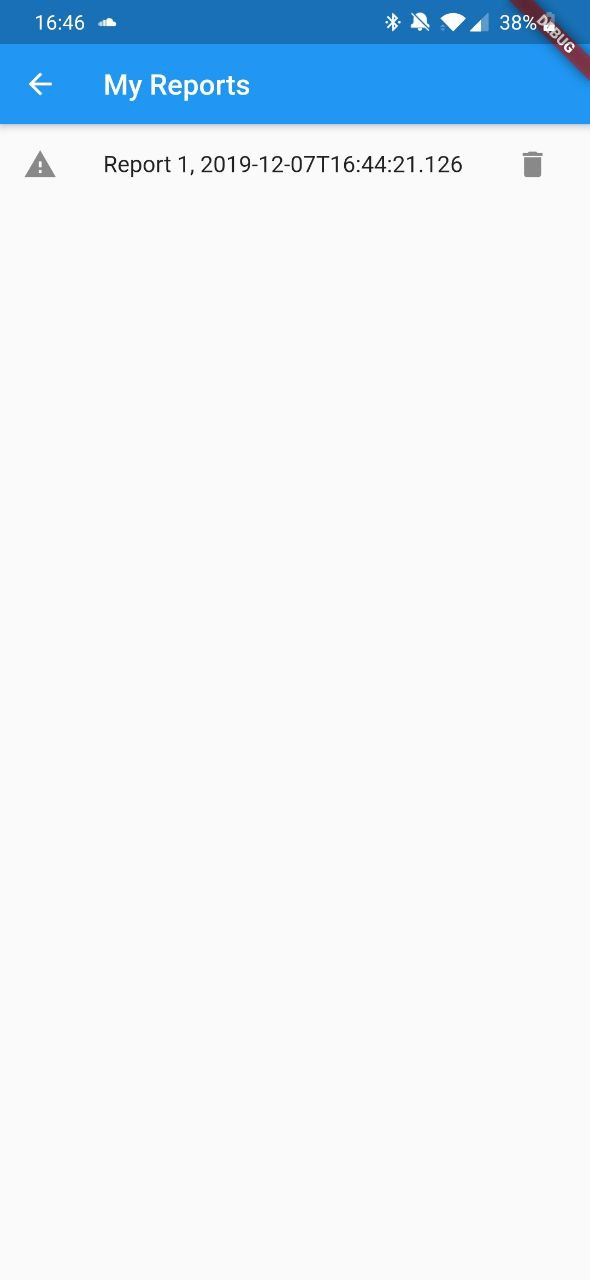
\includegraphics[scale = 0.2]{assets/app_screenshots/myrep.jpg}\\[1.6 cm]
        \caption[\textit{My Reports} Screenshot]{My reports page of SafeStreets.}
    \end{figure}
    \begin{figure}[H]
        \centering
        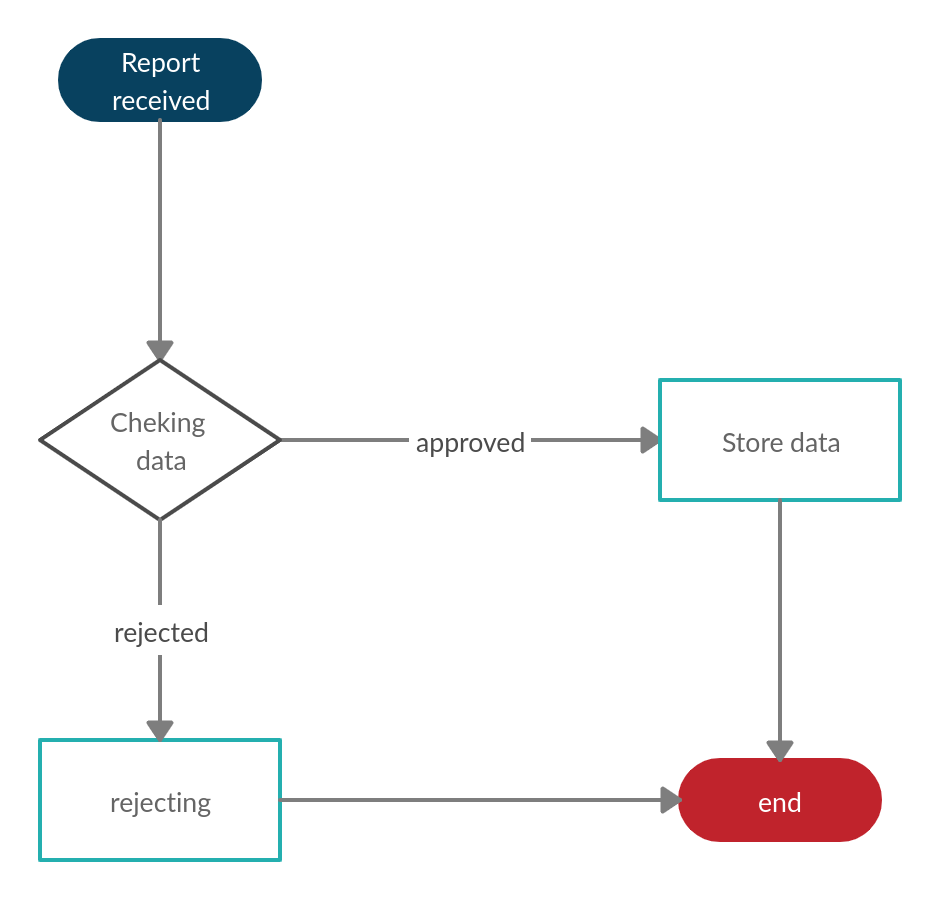
\includegraphics[scale = 0.2]{assets/app_screenshots/report.jpg}\\[1.6 cm]
        \caption[\textit{View Report Citizen} Screenshot]{Report View for a citizen in SafeStreets.}
    \end{figure}
\end{document}